\section{Runtime Results}

%TODO da fare e sistemare.

%\subsection{Tolerance and F1 Score}
We the studied of the influence 
of the tolerance value over the correctness of the algorithms results.
Tests took place on randomly generated automata. A basis of  $\llwb$ was 
computed for each automaton with BPR. An arbitrary number of vector pairs were generated 
as uniformly distributed random linear combinations of the vectors in the spanning set of $\llwb$. 
The same quantity of vector pairs was generated randomly with an uniform distribution.
BPREquivalence and HKC procedures were then executed with those pairs in input.

By defining pairs of vectors as 

\begin{itemize}
    \item \textit{true positives} (TP) if reported as language equivalent by both 
    procedures
    \item \textit{true negatives} (TN) if reported as not language equivalent by both 
    procedures
    \item \textit{false positives} (FP) if reported as language equivalent by HKC but not by BPR
    \item \textit{false negatives} (FN) if reported as  language equivalent by BPR but not by HKC
\end{itemize}


We then borrow four concepts from binary classification: \textit{accuracy, precision, recall} 
and \textit{F1 score}: 

\begin{equation*}
    \begin{aligned}
        \text{Accuracy} = \dfrac{TP + TN}{TP + TN + FP + FN} & \quad & 
        \text{Recall} = \dfrac{TP}{TP + FN} \\ && \\
        \text{Precision} = \dfrac{TP}{TP + FP} & \quad &
        \text{F1} = 2 \cdot \dfrac{\text{Precision} \cdot \text{Recall}}{\text{Precision} + \text{Recall}}  \\ && \\
    \end{aligned}
\end{equation*}

We have then computed 
the F1 score in relation to varying tolerance values.
The plot is shown in Figures \ref{fig:f1} and \ref{fig:f1-2}.  
The program was executed on an x86\_64 AMD Ryzen 5 2600X Six Core CPU, running at 3.6GHz with 32GB RAM, 
running Void Linux. Executed sequentially, F1 score tests took an average 2m26.19s,
Parallelized by using a worker pool, the tests lasted the times reported in 
Figure \ref{fig:f1} and \ref{fig:f1-2}.
For example, in the first plot of Figure \ref{fig:f1-2}, the test took 82 seconds.
Since we computed BPR for 3000 random automata, over 17 tolerance values, for 3 line plots,
with a chance of finding a non-empty basis for $\llwb$ of approximately $1/3$,
the BPR algorithm was executed an approximate average of
$\frac{3000 \cdot 3 \cdot 17}{82} \approx 1865$ times per second. 
The HKC algorithm, was executed 2000 times on each automaton with a non-empty 
basis of $\llwb$, therefore, it was executed an approximate average of 
$\frac{3000 \cdot 17 \cdot 2000 \cdot 3}{3 \cdot 82} \approx 1243902$ times per second.

% //TODO: condizionamento BPR
%TODO: BPR conditioning

\begin{figure}[htbp!]
    \centering
    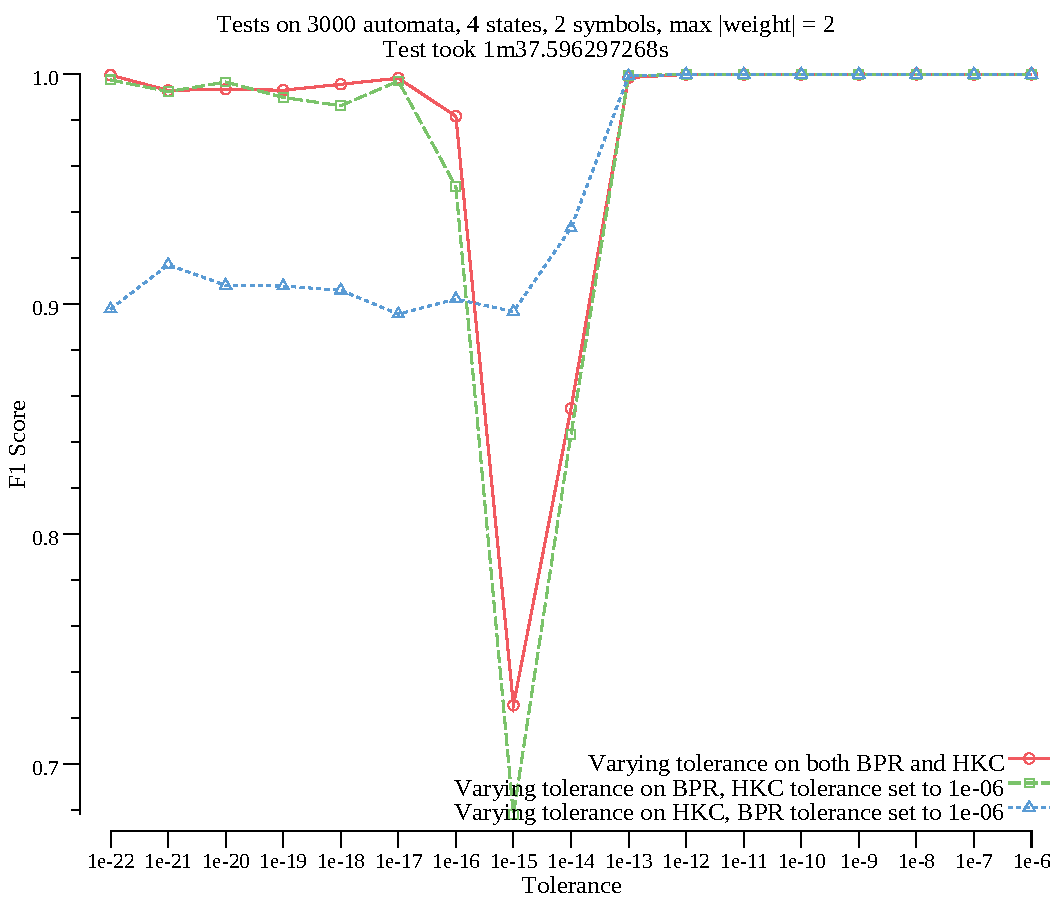
\includegraphics[width=.75\textwidth]{./plots/f1-tol-1e-06.pdf}
    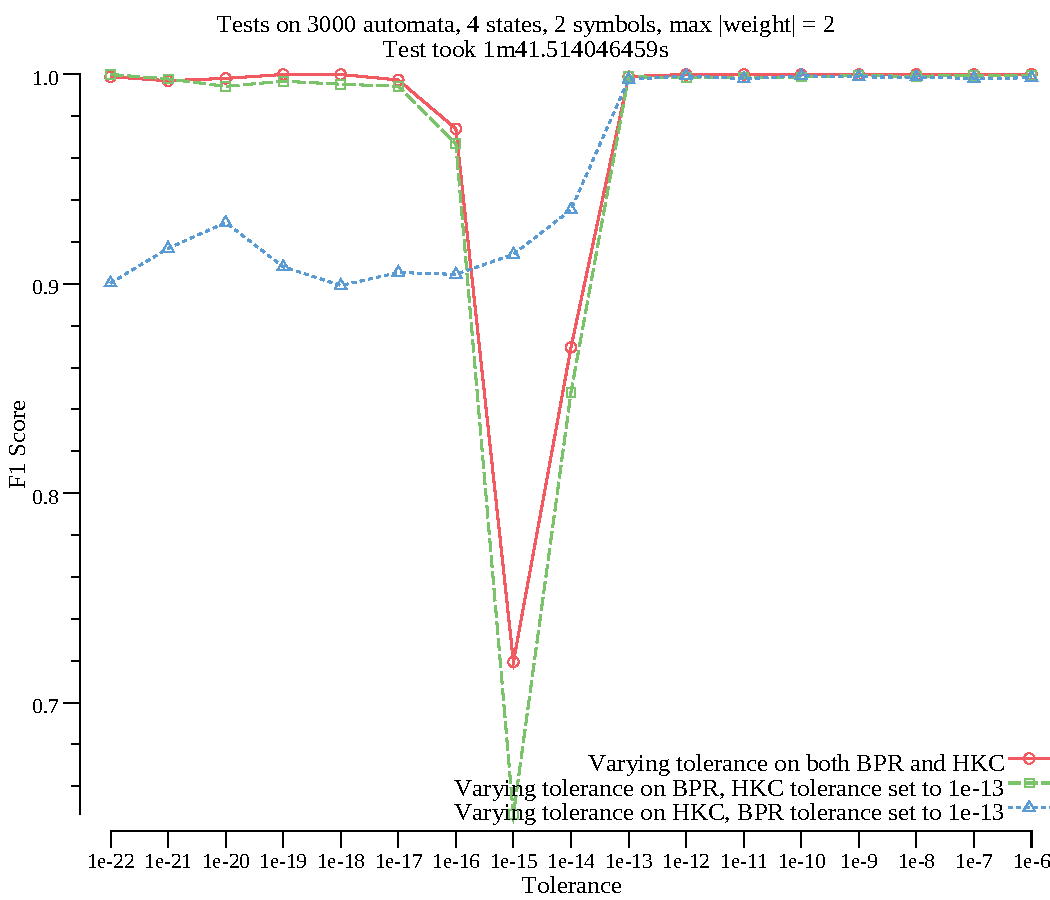
\includegraphics[width=.75\textwidth]{./plots/f1-tol-1e-13.pdf}
    \caption{F1 score over tolerance tests, 2000 vector pairs tested per automaton.}
    \label{fig:f1}
\end{figure}

\begin{figure}[htbp!]
    \centering
    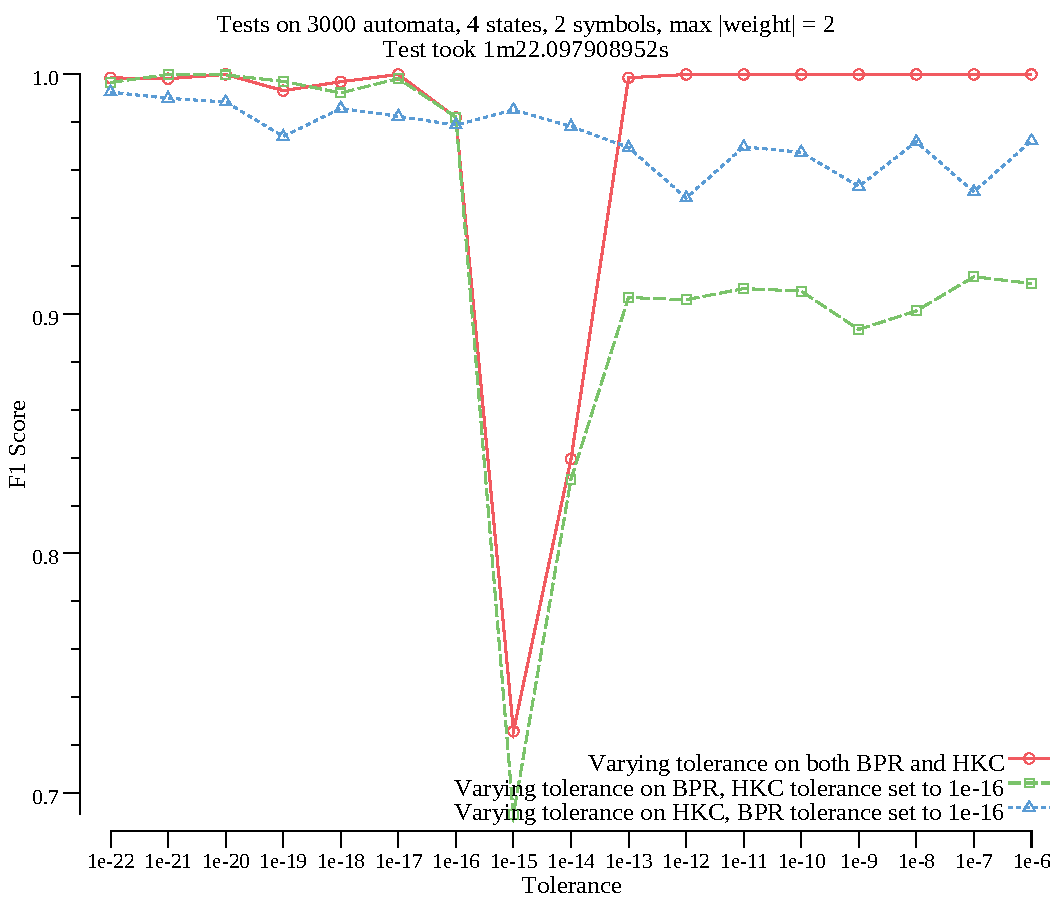
\includegraphics[width=.75\textwidth]{./plots/f1-tol-1e-16.pdf}
    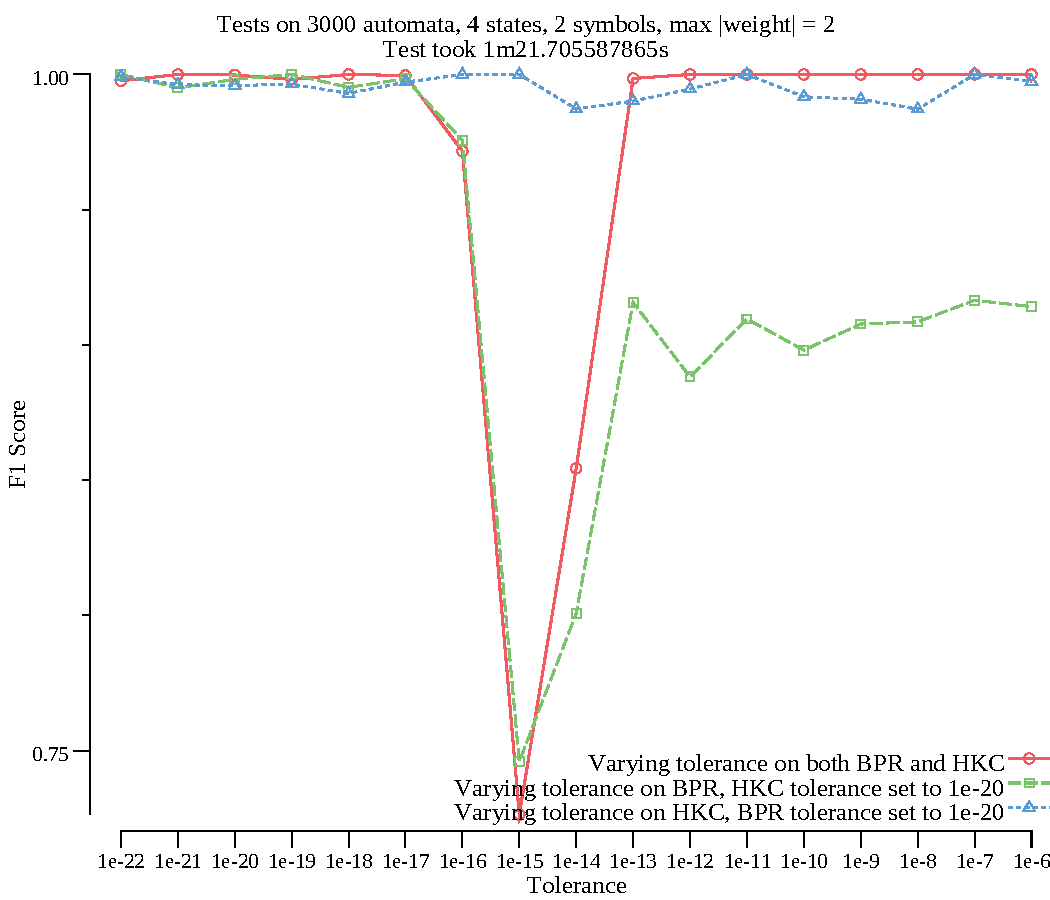
\includegraphics[width=.75\textwidth]{./plots/f1-tol-1e-20.pdf}
    \caption{F1 score over tolerance tests, 2000 vector pairs tested per automaton.}
    \label{fig:f1-2}
\end{figure}


%TODO empty LLWB chance, memory and time plots, varying automata size parameters